%%%%%%%%%%%%%%%%%%%%%%%%%%%%%%%%%%%%%%%%%
% Academic Title Page
% LaTeX Template
% Version 2.0 (17/7/17)
%
% This template was downloaded from:
% http://www.LaTeXTemplates.com
%
% Original author:
% WikiBooks (LaTeX - Title Creation) with modifications by:
% Vel (vel@latextemplates.com)
%
% License:
% CC BY-NC-SA 3.0 (http://creativecommons.org/licenses/by-nc-sa/3.0/)
% 
% Instructions for using this template:
% This title page is capable of being compiled as is. This is not useful for 
% including it in another document. To do this, you have two options: 
%
% 1) Copy/paste everything between \begin{document} and \end{document} 
% starting at \begin{titlepage} and paste this into another LaTeX file where you 
% want your title page.
% OR
% 2) Remove everything outside the \begin{titlepage} and \end{titlepage}, rename
% this file and move it to the same directory as the LaTeX file you wish to add it to. 
% Then add \input{./<new filename>.tex} to your LaTeX file where you want your
% title page.
%
%%%%%%%%%%%%%%%%%%%%%%%%%%%%%%%%%%%%%%%%%

%----------------------------------------------------------------------------------------
%	PACKAGES AND OTHER DOCUMENT CONFIGURATIONS
%----------------------------------------------------------------------------------------

\documentclass[11pt]{article}

\usepackage[utf8]{inputenc} % Required for inputting international characters
\usepackage[T1]{fontenc} % Output font encoding for international characters
\usepackage{graphicx}
\usepackage{mathpazo} % Palatino font
\usepackage[legalpaper,margin=0.9in] {geometry}
\usepackage{fancyhdr}

\setcounter{tocdepth}{4}
\setcounter{secnumdepth}{4}


\pagestyle{fancy}
\fancyhf{}
\lhead{\textsc{University of Regina}}
\rhead{\textsc{Software Systems Engineering}}
\cfoot{\thepage}

\begin{document}

%----------------------------------------------------------------------------------------
%	TITLE PAGE
%----------------------------------------------------------------------------------------

\begin{titlepage} % Suppresses displaying the page number on the title page and the subsequent page counts as page 1
	\newcommand{\HRule}{\rule{\linewidth}{0.5mm}} % Defines a new command for horizontal lines, change thickness here
	
	\center % Centre everything on the page
	
	%------------------------------------------------
	%	Headings
	%------------------------------------------------
	
	\textsc{\Huge University of Regina}\\[1.5cm] % Main heading such as the name of your university/college

	\textsc{\Large ENSE 477: Software Capstone Project}\\[0.5cm]
	
	\textsc{\Large Software Systems Engineering}\\[0.5cm] % Major heading such as course name
	
	
	
	
	%------------------------------------------------
	%	Title
	%------------------------------------------------
	
	\HRule\\[0.4cm]
	
	{\Huge\bfseries Workshop Enterprise Resource Planning Suite Resources and Specifications Document}\\[0.4cm] % Title of your document
	
	\HRule\\[1.5cm]
	
	%------------------------------------------------
	%	Author(s)
	%------------------------------------------------
	
	\begin{minipage}[t]{0.4\textwidth}
		\begin{flushleft}
			\large
			\textsc{Authors}\\
			Jonathan Wells\\
			\textsc{200328640}\\ % Your name
			\large
			Konstantin Kharitonov\\
			\textsc{200354502} % Supervisor's name
		\end{flushleft}
		
	\end{minipage}
	~
	\begin{minipage}[t]{0.4\textwidth}
		\begin{flushright}
			\large
			\textsc{Supervisor}\\ % Supervisor's name
			Karim Naqvi\\
			M. A.Sc., P.Eng.\\
		\end{flushright}
	\end{minipage}
	
	% If you don't want a supervisor, uncomment the two lines below and comment the code above
	%{\large\textit{Author}}\\
	%John \textsc{Smith} % Your name
	%------------------------------------------------
	%	Logo
	%------------------------------------------------
	
	\vfill\vfill\vfill\vfill
	
\includegraphics[width=0.7\textwidth]{UR.png}\\[2cm] % Include a department/university logo - this will require the graphicx package
	 

	%------------------------------------------------
	%	Date
	%------------------------------------------------
	
	\vfill\vfill\vfill % Position the date 3/4 down the remaining page
	
	{\large\today} % Date, change the \today to a set date if you want to be precise
	
	%----------------------------------------------------------------------------------------
	
	\vfill % Push the date up 1/4 of the remaining page
	
\end{titlepage}

%----------------------------------------------------------------------------------------

%----------------------------------------------------------------------------------------
%Table of Contents %

\newpage 
\tableofcontents
%-------------------------------------------------------------------------------------

%-------------------------------------------------------------------------------------
%Table of Figures % 
\newpage
\listoffigures

%-------------------------------------------------------------------------------------
%Introduction%
\newpage
\section{Introduction}
The Workshop Enterprise Resource Planning Suite, or ERP for short, is an administrative task management web application primarily designed for the Engineering Workshop at University of Regina main campus. It is to be the main application to be used for managing incoming and outgoing workorders, which are student and faculty submitted forms requesting the service of the shop. The service provides workorder capacity planning, allowing for the user to actively manage the status of each project, time tracking features for large scale and small scale work, as well as the ability to track the inventory of the workshop, including but not limited to, materials, tools and equipment. 
\subsection{Purpose}
This system was designed to replace the previous methods of workorder, time, and inventory tracking, centralizing all aspects into one powerful application that can be accessed online. Workorders currently must be submitted via paper form directly to the workshop during its operating hours. The form must then be reviewed by the workshop manager and if accepted, future meetings are scheduled. All workorders submitted are then stored physically in binders, which date back to the opening of the workshop. All materials and inventory are also stored physically. This project intends to automate all workorders and have then be submitted and archived electronically. As well, the system is intended to track all scopes of projects, ranging from small miscellaneous tasks to larger scale projects in such a fashion that the workshop manager can schedule them effectively in advance. 
\subsection{Scope}
ERP is designed as a Web API, such that it is run in browser and is able to be accessed from any computer with a sufficient internet connection. It will be a local application that will be primarily accessed by the workshop manager, who is this project's main client. Secondary clients include faculty and staff that wish to submit workorders over the ERP suite. The primary client is the only one intended to have full control of all features of the ERP suite. 
\newline
{\setlength{\parindent}{0cm}

The ERP Suite currently is planned to be exclusive to the engineering workshop based on its design as of the completion of this capstone project, as future work on this project will require a redesign to be re-purposed for future clients. The ideal future client for this program is for machine and workshop owners with a staff less than 50.  

\newpage

\section{Overall Description}
\subsection{Product Perspective}
The Workshop ERP suite is broken up into its 3 main functionalities: 

	\begin{enumerate}
	\item Workorders
	\item Time Tracking and Project Management 
	\item Inventory
	\end{enumerate}

Each feature can be accessed from the navigation side bar, which is present on all pages of the web application. 

\subsubsection*{Workorders:}
On the workorder page, the client is able to access all workorders currently present in the system, whether they be first or historical submissions. Options include but not limited to, viewing user submissions, filter through all workorders, and tag them based on progress status and importance. The following figure showcases the different stages of a workorder throughout the submission process.
 
\begin{figure}[h]
	\centering
	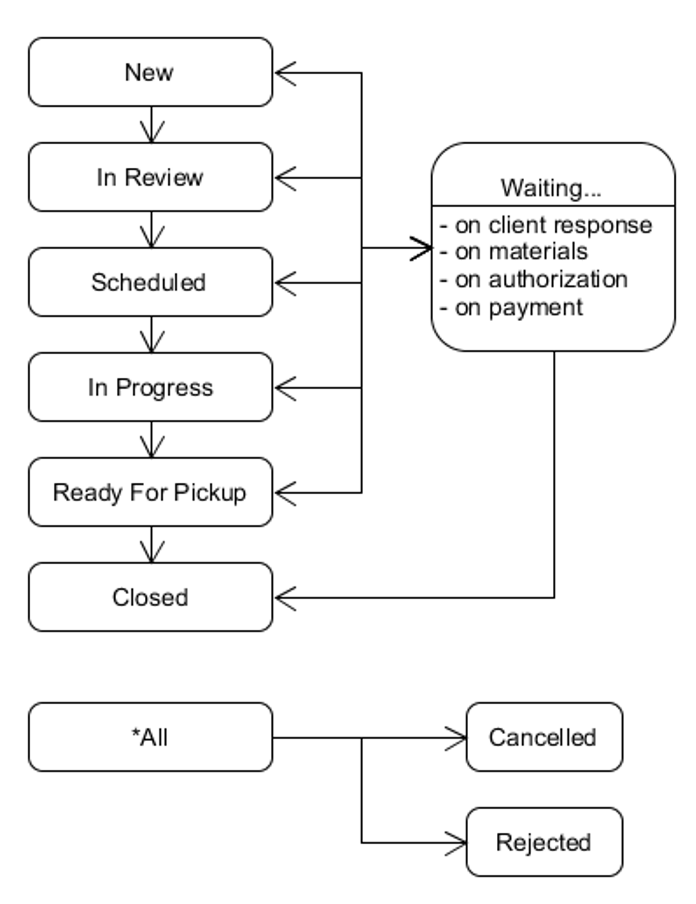
\includegraphics[width=5in]{workorder-status.png}\\
	\caption{Different Stages of a Workorder}
	\label{fig:tobias}
\end{figure}

\subsubsection*{Time Tracking and Project Management:}
This page includes all of the time tracking features such as submitting current activities/projects into the system's calendar and creating a plan for workorders to be completed in the future. The time tracking page is also used for an accurate description of each semester, highlighting which project was worked each day. Functionality from this feature is also shown on the right navigation bar, allowing for quick access to daily tasks and which project deadlines are approaching the current date.

\subsubsection*{Inventory:}
The inventory page is where the client is able to access and filter through the materials that are currently or previous were in stock in the workshop. Each material is able to be found inside the inventory database, as well as describing each based on filters such as type, amount, and length. Vendor information from where the material was purchased from and price per pound is also accessed from here. 

\subsection{Constraints}
As currently designed, the program is intended to only be used on campus. It is specific to the engineering workshop on campus and must go through a redesign before it can be distributed to a different client. As well, a steady internet connection is required to access the application as well as connect to the server hosting the application and its associated databases. The service is not optimised to mobile and as such, the user is heavily encouraged to the desktop version, though it is not a complete necessity.  
\newline
{\setlength{\parindent}{0cm}

Some non-technical restraints include the application being unilingual to English, must be follow university guidelines of conduct, and requires a basic understanding of computing.  

\subsection{Operating Enviroment}
The project is split into two main categories for development; the frontend and the backend. 
\newline
{\setlength{\parindent}{0cm}

The frontend implements the Vue.js framework based upon javascript. It is an online front end framework that allows developers to build user interfaces and single page web applications. For development, the frontend ran on a development localhost server which allowed for dynamic programming and error-checking. SCSS is also used to add functionality to CSS pages.  
\newline
{\setlength{\parindent}{0cm}

The backend is ASP.NET, Microsoft's own open-source server side web application framework, using the C\# language. The project is also optimized to use Entity Framework.Databases are stored and accessed through a SQL server which is connected to the backend.
\newline
{\setlength{\parindent}{0cm}

Visual Studio Code is used as the primary code editor for all frontend development. Visual Studio is used for server side and database programming. Google Chrome the browser interface that is currently used during implementation. 

\subsection{Dependencies}
For the ERP suite function to provide the most value to the client, all data submitted inside application must be accurate, as the system will only perform based on the data that is given to the system. Workorders are assumed to be submitted in the proper predefined format such that crucial data is not lost throughout the project's lifetime. If a redesign of the workorder format is needed, documentation of this change is highly recommended.
\newline
{\setlength{\parindent}{0cm}
 
As well, all materials submitted into the inventory page must be properly accounted for in shop as well as on site. The program will display the information that it will receive, and changes to any inventory should be recorded as is necessary. The system relies on the user to file inventory data frequently to be considered up to date. 
\newline
{\setlength{\parindent}{0cm}

Since this application is currently being  developed in Sasktachewan, the system will use Staskatchewan standard time and will not account for any daylight savings that may occur if the program is used elsewhere in the work. 
\section{System Features}

\section{External Interface Requirements}
\section{Non-Functional Requirements}
\section{References}


\end{document}
